\documentclass[10pt,a4paper]{article}
\usepackage[margin=2.1cm]{geometry}
\usepackage{amsmath,amssymb,bm}
\usepackage{graphicx,booktabs,xcolor,enumitem,hyperref}
\hypersetup{colorlinks,linkcolor=blue!50!black,urlcolor=blue!50!black}
\newcommand{\ka}{\kappa_1}
\newcommand{\kc}{\kappa_2}
\newcommand{\note}[1]{\par\smallskip\noindent\colorbox{gray!12}{\parbox{\dimexpr\linewidth-2\fboxsep}{\small #1}}\par\smallskip}
\newcommand{\evd}[1]{\textsf{\small[#1]}}
\newcommand{\simple}[1]{\par\noindent\textbf{In simple words:} #1\par\smallskip}
\title{TOP-Q --- Day 5 worked notes\\[2pt]\large Light propagation, what ``the phase'' means, and loss}
\author{PH 5110 term paper --- Kotapati Kishore (EE26E016)}
\date{31 October 2026 (done one day ahead of the revised plan)}
\begin{document}\sloppy\maketitle

\note{All results are \textbf{numerical simulations} \evd{Simulated} unless marked \evd{Derived}. Arrays T and D as on Day 3, now with $M=81$ guides so that no light reaches the ends before the output (largest edge power before $z=L$: $6\times10^{-13}$). Device length $L=5\pi/\kc$ = \textbf{10 coupling lengths} $\pi/(2\kc)$, the minimum suggested by Blanco-Redondo \emph{et al.} Units: $z$ in $1/\kc$, $b$ and $\alpha$ in $\kc$.}

\tableofcontents

%=====================================================================
\section{How light moves through the array}
%=====================================================================
\subsection{The propagator \evd{Derived}}
From $d\bm a/dz=iH\bm a$: $\bm a(z)=U(z)\bm a(0)$ with $U(z)=e^{iHz}$. Writing $H=\sum_m b_m\psi_m\psi_m^\dagger$,
\[
\bm a(z)=\sum_m\underbrace{\langle\psi_m|\bm a(0)\rangle}_{\text{how much of mode }m}\;e^{ib_mz}\;\psi_m .
\]
\simple{split the input light into the array's modes; each mode just turns its phase at its own speed $b_m$; add them back up at the output.}

\textbf{Code checks} \evd{Verified-by-test}: $U$ is unitary and $U(z_1)U(z_2)=U(z_1+z_2)$; total power stays 1 to $10^{-12}$; results agree with an independent ODE solver (SciPy \texttt{solve\_ivp}, 8th-order Runge--Kutta) to $10^{-8}$, with and without loss.

\subsection{Launching into the centre guide}
Putting all light into the centre guide $c$ sends a fraction $|\psi_0(c)|^2$ into the defect mode. For both T and D this is $(1-r^2)/(1+r^2)=0.8$ \evd{Derived; Verified-by-test} --- the IPR matching of Day 3 also makes the launch efficiency equal. The other 20\% goes into bulk modes and spreads out (Fig.~\ref{fig:prop}a,b).
Fig.~\ref{fig:prop}c: light put into the guide \emph{next to} the T centre does not excite the zero mode at all (the zero mode is exactly zero there) and walks away. Fig.~\ref{fig:prop}d: a uniform array shows pure \textbf{discrete diffraction}, two outgoing lobes --- the same pattern Blanco-Redondo \emph{et al.} measured for their equidistant reference array \evd{Literature}.

\begin{figure}[t]\centering
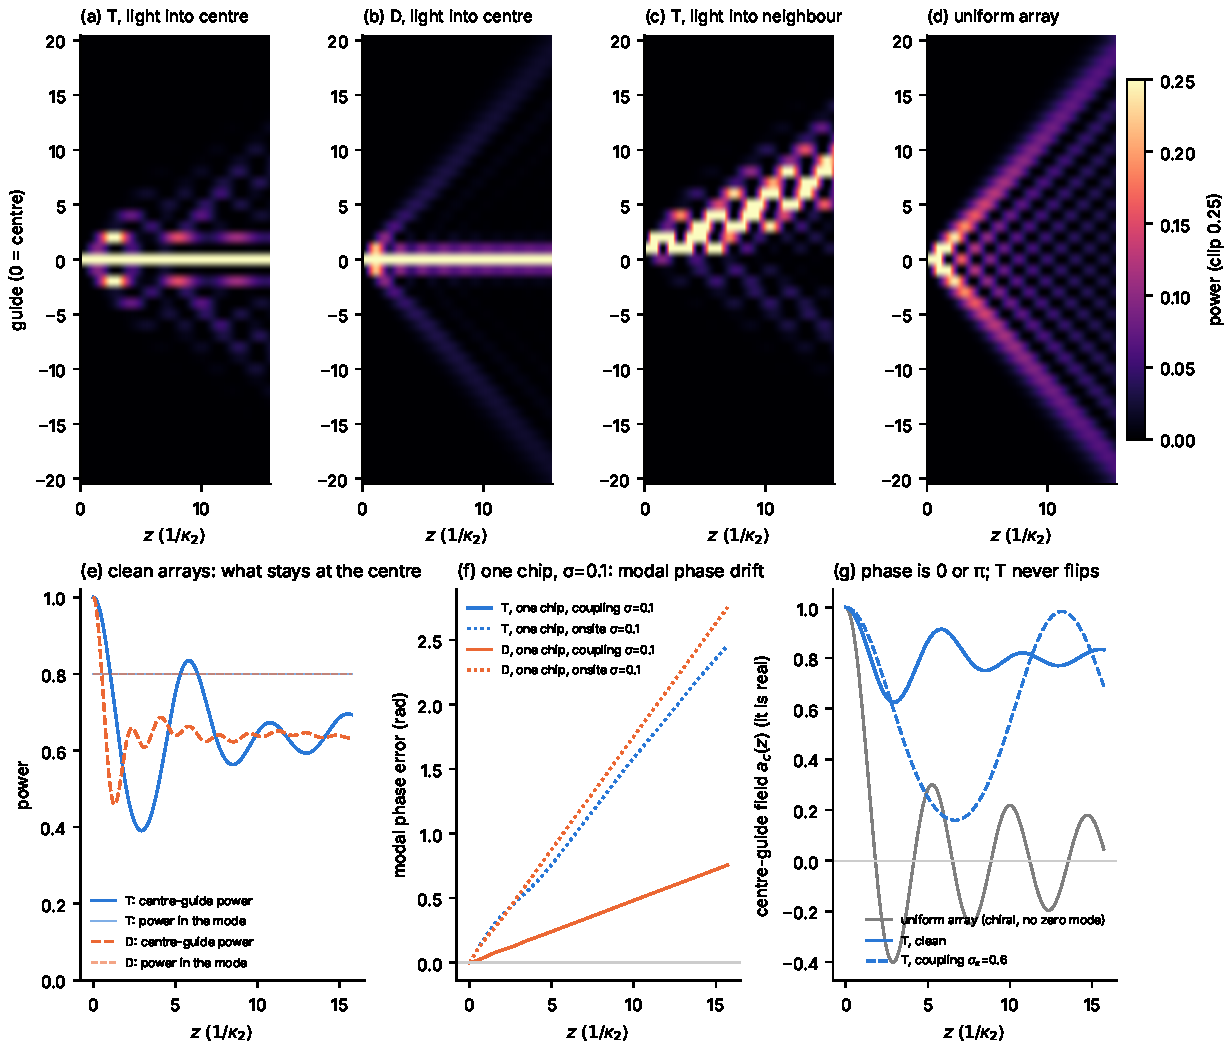
\includegraphics[width=\linewidth]{../../figures/fig_propagation.pdf}
\caption{\textbf{Simulation}, generated by \texttt{scripts/day5\_propagation.py} from \texttt{data/day5\_propagation.npz}. (a)--(d) Power in each guide vs.\ $z$ (top views, like a fluorescence image). (e) Power left in the centre guide and power in the defect mode. (f) Phase error of the defect-mode amplitude on one disordered chip ($\sigma=0.1$). (g) The centre-guide field: always real; only T never changes sign.}
\label{fig:prop}
\end{figure}

%=====================================================================
\section{What do we mean by ``the phase''?}
%=====================================================================
There are (at least) two honest definitions, and they answer different questions:\par\smallskip\noindent
\begin{tabular}{@{}p{0.2\linewidth}p{0.36\linewidth}p{0.36\linewidth}@{}}\toprule
 & \textbf{Modal phase} $\varphi_{\rm m}=\arg\langle\psi_0|\bm a(L)\rangle$ & \textbf{Output-guide phase} $\varphi_{\rm g}=\arg a_c(L)$\\\midrule
What it is & phase of the light that is in the defect mode & phase of the light in the centre output guide\\
Who sees it & a perfect mode filter & an interferometer that taps that one guide\\
Clean value & $b_0L$ (T: 0; D: $\tfrac{20}{9}L$) & $b_0L$ + small wiggles from bulk light\\\bottomrule
\end{tabular}
\smallskip

Both are measured \textbf{relative to $\beta_0L$}. The common term $\beta_0L$ is the same for every guide and cancels when two arms share it. The phase \emph{error} we care about is (disordered chip) $-$ (clean chip) at $z=L$. To first order, $\delta\varphi_{\rm m}\approx\delta b\,L$: \textbf{the phase error grows in proportion to the length}. Fig.~\ref{fig:prop}f, one chip with on-site $\sigma_\beta=0.1$: T drifts by 2.4~rad and D by 2.7~rad over 10 coupling lengths. With coupling disorder, T does not drift at all; D drifts by 0.76~rad.

%=====================================================================
\section{A new result: chiral symmetry makes the phase 0 or $\pi$}
%=====================================================================
\subsection{The theorem \evd{Derived; Verified-by-test}}
Launch in guide $c$ and look at the same guide. Then
\[
a_c(z)=\langle c|e^{iHz}|c\rangle=\sum_m|\psi_m(c)|^2e^{ib_mz}.
\]
If $H$ is chiral, the modes come in pairs $\psi_m$ and $\Gamma\psi_m$ with $b\to-b$, and $|\Gamma\psi_m(c)|=|\psi_m(c)|$. Each pair adds $|\psi_m(c)|^2(e^{ibz}+e^{-ibz})=2|\psi_m(c)|^2\cos bz$, which is \emph{real}. So
\[
\boxed{a_c(z)\ \text{is real for every }z\text{ in ANY chiral array}\ \Rightarrow\ \varphi_{\rm g}\in\{0,\pi\}.}
\]
Numerically $|\mathrm{Im}\,a_c|<3\times10^{-15}$ for the uniform array, clean T, and T with $\sigma_\kappa=0.6$.

\subsection{What topology adds: no sign flip}
The zero mode contributes a constant $w_0=|\psi_0(c)|^2$, and all the rest together has size at most $1-w_0$, so
\[
\mathrm{Re}\,a_c(z)\ \ge\ 2w_0-1 .
\]
If $w_0>1/2$, the field can never cross zero, so the phase stays at 0 at \emph{every} length. Clean T: $w_0=0.8$, so $a_c\ge0.6$ (measured minimum 0.62). The uniform array is also chiral but has no zero mode: its field swings negative (minimum $-0.40$), so its phase jumps between 0 and $\pi$ (Fig.~\ref{fig:prop}g).
\note{\textbf{This is the cleanest answer so far to the research question.} For a chiral array, \emph{chiral symmetry alone} (not topology) forces the self-phase to be 0 or $\pi$. \emph{Topology} (the zero mode) is what keeps it at 0 rather than flipping, \emph{as long as} the zero mode keeps more than half of its weight on the input guide. Day 4 showed this weight falls to 0.61 at $\sigma_\kappa=0.6$ and 0.54 at 0.8 --- close to the 0.5 limit. And all of this fails the moment chiral symmetry is broken (on-site errors).}

%=====================================================================
\section{Loss}
%=====================================================================
\subsection{Uniform loss \evd{Derived; Verified-by-test}}
Power loss $\alpha$ per unit length: $H\to H+i\frac{\alpha}{2}\mathbb1$. Because $\mathbb1$ commutes with $H$, $\bm a(z)=e^{-\alpha z/2}\times$(lossless result): \textbf{power drops as $e^{-\alpha z}$ and every phase is unchanged} (measured change $\le2\times10^{-14}$ rad, Fig.~\ref{fig:loss}a).

\subsection{Random loss: the zero mode's phase is still pinned \evd{Derived; Verified-by-test}}
Let each guide have its own loss: $H=H_0+iD$, with $D$ real and diagonal and $H_0$ chiral. Then
\[
\Gamma H\Gamma=-H_0+iD=-(H_0-iD)=-H^\dagger .
\]
This forces the eigenvalues into pairs $(b,\,-b^*)$. A single isolated mode must be its own partner: $b=-b^*$, i.e.\ $\mathrm{Re}\,b=0$ \emph{exactly}. Its \emph{decay} ($\mathrm{Im}\,b$) changes, but its \emph{phase velocity} does not.
Numbers (500 chips per point, loss uniformly random in $[0,2\bar\alpha]$): T: std of $\mathrm{Re}\,\delta b\approx10^{-15}$ for all $\bar\alpha$; D: $10^{-6}$ to $10^{-3}$ (a second-order effect). Both lose amplitude at the same average rate $\approx\bar\alpha/2$ (Fig.~\ref{fig:loss}b).
\evd{Literature: the idea of a zero mode surviving in a lossy SSH lattice was demonstrated in waveguides by Weimann \emph{et al.}, Nature Materials \textbf{16}, 433 (2017), doi:10.1038/nmat4811 --- read it before citing for this exact statement.}

\simple{loss makes the light dimmer. Uniform loss dims everything equally and changes no phases. Random loss also makes the topological mode dimmer by a random amount, but it still does not change its phase. So for T, loss turns into an \emph{amplitude} error, not a phase error. For an interferometer, an amplitude error between the two arms still lowers the contrast (Day 8).}

\begin{figure}[h]\centering
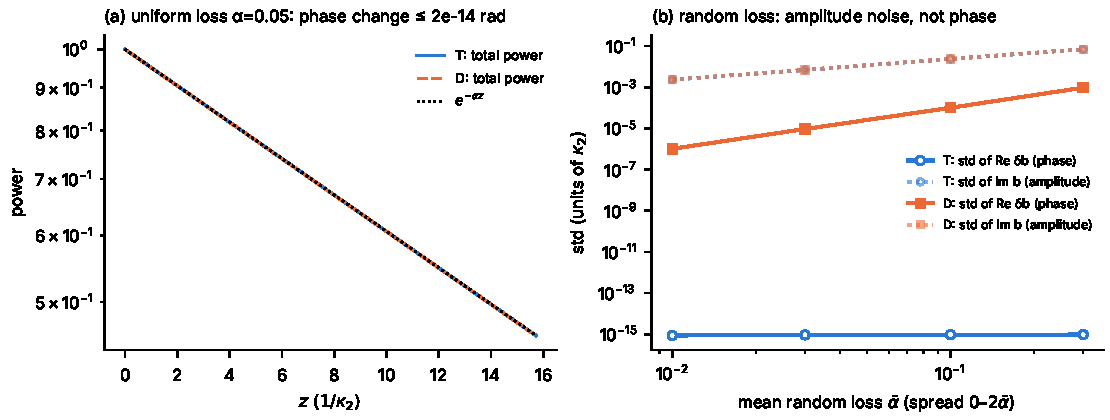
\includegraphics[width=\linewidth]{../../figures/fig_loss.pdf}
\caption{\textbf{Simulation} (\texttt{data/day5\_propagation.npz}). (a) Uniform loss: pure exponential, no phase change. (b) Random loss: spread of the phase rate $\mathrm{Re}\,\delta b$ (solid) and of the decay rate $\mathrm{Im}\,b$ (dotted). T's phase rate is pinned at round-off level.}
\label{fig:loss}
\end{figure}

%=====================================================================
\section{Five different things --- now with evidence}
%=====================================================================
\begin{tabular}{@{}p{0.22\linewidth}p{0.36\linewidth}p{0.34\linewidth}@{}}\toprule
Property & Protected by & Broken by\\\midrule
Eigenvalue pinning ($b=0$) & chiral symmetry (exact) & on-site / width errors\\
Localisation at the input & topology + gap; weakens with strong disorder & strong coupling disorder (Day 4)\\
Self-phase $\in\{0,\pi\}$ & \textbf{chiral symmetry alone} & on-site / width errors\\
Self-phase $=0$ (no flip) & topology: zero-mode weight $w_0>1/2$ & $w_0<1/2$; on-site errors\\
Phase rate under random loss & non-Hermitian chiral pairing $(b,-b^*)$ & on-site errors\\
Transmitted power & nothing special: same mode loss as D & loss of any kind\\\bottomrule
\end{tabular}

%=====================================================================
\section{Hardware: how propagation and loss are measured in real labs}
%=====================================================================
\textbf{We did none of these measurements.} The images shown in our chat (from published papers) illustrate the real methods:
\begin{itemize}[itemsep=1pt]
\item \textbf{Top-view imaging of light inside an array.} In femtosecond-laser-written glass waveguides, light scattered or fluoresced from the waveguides is filmed from above; the pictures look like our Fig.~\ref{fig:prop}a--d. Silicon chips cannot be viewed this way easily, so only the output is seen.
\item \textbf{Output-facet imaging.} The light leaving the chip edge is focused onto an infrared camera; each bright spot is one waveguide. This gives $|a_n(L)|^2$ but \emph{not} the phase. To get a phase, the output must interfere with a reference beam --- i.e.\ an interferometer, which is exactly why Days 8--10 build MZIs.
\item \textbf{Cut-back loss measurement.} Measure the transmitted power for several waveguide lengths and fit a straight line on a log scale; the slope is $\alpha$. This is the experimental version of Fig.~\ref{fig:loss}a.
\end{itemize}
Look up and cite the source papers shown with each image before using them (``Reproduced from [ref]'').

\section{Code and tests}
New: \texttt{topq/propagation.py} (loss, propagator, propagate, launch, modal amplitude, guide field), \texttt{scripts/day5\_propagation.py}, \texttt{tests/test\_propagation.py} (15 tests, including the real-amplitude theorem, the $2w_0-1$ bound and the loss pinning). Suite: \textbf{93 passed}. Run time of the script: about 30~s.

\section{Self-test}
\begin{enumerate}[itemsep=1pt]
\item Why does light launched next to the T centre not excite the zero mode?
\item Prove in three lines that $a_c(z)$ is real in a chiral array.
\item Why does the uniform array's centre field change sign but T's does not?
\item Why does uniform loss change no phase?
\item Show that $\Gamma(H_0+iD)\Gamma=-(H_0+iD)^\dagger$ forces $\mathrm{Re}\,b=0$ for an isolated mode.
\item Why does a longer device make phase errors worse?
\end{enumerate}
\end{document}
